
%%%
% Discussion of how each strategy was used as a separate starting point
%%%

\subsubsection*{Starting Points}
\label{sec:findings-expts-starts}

%%%
Since a desired outcome of the learning process was to be able to use the
generated strategy graphs to tell how a hand \textit{should} be played in a
certain score position,
a comparison was made between the produced agent and pure strategies
on a database of choices made by humans.
%
There exists a website in which users are prompted with a set of dealt cards and
a given score and must decide which set of cards they would keep in that
specific situation
\cite{dailycribbagehand}.
%%%

%%%
With access to recorded answers,
the agent's choices could be compared to how humans ranked the choice.
%
The retrieved database recorded which responses were given to each query
and could be used to determine how well the agent's choice matched with those
made by humans in the same situation.
%
For each of the more than 3600 usable records,
the choice the agent made was compared against those made by the users of the
website.
%
The results of this comparison can be seen in
Table~\ref{tab:expts-starts-human}. % TODO: ref more tables if created
%%%

%%%
Table~\ref{tab:expts-starts-human} shows that the trained agent chooses the same
set of cards as the human users only marginally more often than an agent with 
randomly allocated weights.
%
In approximately half of the cases,
the trained agent chooses the same answer as most humans;
in almost 78 percent of the cases,
the answer given by the agent is within the top three most common human answers.
%
Additionally,
most pure strategies,
created by setting their weight to 1 while all others are 0,
performed worse than the trained mixture.
%
Notable exceptions to this trend are the \handmaxposs\ and \handmaxavg\ 
strategies,
suggesting that in more situations than the agent,
the typical human player will play more according to what points can be expected
to be gained from the cut card.
%
Interestingly,
the \handmaxposs\ strategy's presence as the second most common pure strategy
used indicates a significant degree of risk-taking present in the users'
responses.
%%%

%%%
As a result of this finding,
each of these strategies were used as initial weights to the learning process
in order to determine if the agent could learn to fine-tune a policy starting
from a reasonable assertion of good game-play
as well as learn to discount demonstrably poor strategies.
%
Since the update mechanism for weights relies upon renormalization of a vector
which as been rewarded or punished,
no modifications would occur in the case of punishment of a pure strategy
since no other weights would have the chance to increase.
%
Therefore,
the pure strategies used before were slightly modified so that each other
element of the \wvec\ vector would have a small initial value which would be
increased when the pure strategy was punished.
%%%


\begin{table}

	\begin{tabular}{|r|c|c|c|p{4cm}|}
		\hline
		\textbf{Strategy} & \textbf{Top 1} & \textbf{Top 2} & \textbf{Top 3}
			& \textbf{Percentage in Top 3 Human Choices} \\
		\hline
		\peggingminavggiven & 160 & 303 & 458 & 12.64 \\\hline
		\peggingmaxmedgained & 268 & 519 & 796 & 21.97 \\\hline
		\peggingmaxavggained & 347 & 650 & 963 & 26.58 \\\hline
		\cribminavg & 380 & 177 & 1081 & 29.84 \\\hline
		\handmaxmin & 1576 & 2288 & 2666 & 73.59 \\\hline
		\textbf{Random} & \textbf{1581} & \textbf{2318} & \textbf{2759} &
			\textbf{76.15} \\\hline
		\handmaxmed & 1649 & 2353 & 2768 & 76.40 \\\hline
		\textbf{Trained} & \textbf{1706} & \textbf{2426} & \textbf{2821} &
			\textbf{77.86} \\\hline
		\handmaxposs & 1677 & 2433 & 2847 & 78.58 \\\hline
		\handmaxavg & 2066 & 2828 & 3168 & 87.44 \\\hline
	\end{tabular}
	% total = 3623
	\caption{
		Number of times the agent using a given strategy chose the same cards as
		the most common choice by human users
		according to 3623 total parsable records obtained from
		\cite{dailycribbagehand}.
		The columns labeled ``Top X'' display the number of times the given
		strategy's choice was within the top X choices of the user base.
		%if at least that many different choices were made
		In this table,
		\textbf{Random} is from the best result of five agents which each used
		independently randomly allocated weights
		and
		\textbf{Trained} uses an agent trained from Round 2 for one million
		games.
	}
	\label{tab:expts-starts-human}
\end{table}



\paragraph*{Results}

% fig:findings-expts-sanitycheck-matrix
\begin{figure}
\centering

\begin{tabular}{ l l l l l l } %    c}
	%                    label
	%  l            | l1   l2   l3   l4
	%  a   ---------+-------------------
	%  b   starting | a1 | a2 | a3 | a4
	%  e   strat    | b1 | b2 | b3 | b4
	%  l   ...
	& & \multicolumn{4}{c}{\textit{Strategy}} \\
	& & \handmaxmin & \handmaxavg & \handmaxposs & \handmaxmed \\
	%\cline{3-6}
	\multirow{7}{*}{
	\rotatebox{90}{
	\parbox[c]{6.5cm}{
		\textit{Starting Strategy}
	}
	}
	}
	%
	& \rotatebox[origin=c]{90}{\handmaxmin}
		&\parbox[c]{1em}{
\includegraphics[width=2.5cm]{images/findings/experiments/starting_points/matrix_handmaxmin_handmaxmin.png}}
		&\parbox[c]{1em}{
\includegraphics[width=2.5cm]{images/findings/experiments/starting_points/matrix_handmaxmin_handmaxavg.png}}
		&\parbox[c]{1em}{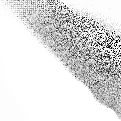
\includegraphics[width=2.5cm]{images/findings/experiments/starting_points/matrix_handmaxmin_handmaxposs.png}}
		&\parbox[c]{1em}{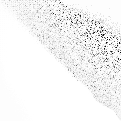
\includegraphics[width=2.5cm]{images/findings/experiments/starting_points/matrix_handmaxmin_handmaxmed.png}}
		%&
	\\ & & & & & \\
	%
	& \rotatebox[origin=c]{90}{\handmaxavg}
		&\parbox[c]{1em}{
\includegraphics[width=2.5cm]{images/findings/experiments/starting_points/matrix_handmaxavg_handmaxmin.png}}
		&\parbox[c]{1em}{
\includegraphics[width=2.5cm]{images/findings/experiments/starting_points/matrix_handmaxavg_handmaxavg.png}}
		&\parbox[c]{1em}{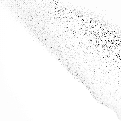
\includegraphics[width=2.5cm]{images/findings/experiments/starting_points/matrix_handmaxavg_handmaxposs.png}}
		&\parbox[c]{1em}{
\includegraphics[width=2.5cm]{images/findings/experiments/starting_points/matrix_handmaxavg_handmaxmed.png}}
		%&\parbox[c]{1em}
	\\& & & & & \\
	%
	& \rotatebox[origin=c]{90}{\handmaxposs}
		&\parbox[c]{1em}{
\includegraphics[width=2.5cm]{images/findings/experiments/starting_points/matrix_handmaxposs_handmaxmin.png}}
		&\parbox[c]{1em}{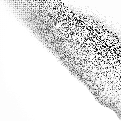
\includegraphics[width=2.5cm]{images/findings/experiments/starting_points/matrix_handmaxposs_handmaxavg.png}}
		&\parbox[c]{1em}{
\includegraphics[width=2.5cm]{images/findings/experiments/starting_points/matrix_handmaxposs_handmaxposs.png}}
		&\parbox[c]{1em}{
\includegraphics[width=2.5cm]{images/findings/experiments/starting_points/matrix_handmaxposs_handmaxmed.png}}
		%&\parbox[c]{1em}
	\\& & & & & \\
	%
	& \rotatebox[origin=c]{90}{\handmaxmed}
		&\parbox[c]{1em}{
\includegraphics[width=2.5cm]{images/findings/experiments/starting_points/matrix_handmaxmed_handmaxmin.png}}
		&\parbox[c]{1em}{
\includegraphics[width=2.5cm]{images/findings/experiments/starting_points/matrix_handmaxmed_handmaxavg.png}}
		&\parbox[c]{1em}{
\includegraphics[width=2.5cm]{images/findings/experiments/starting_points/matrix_handmaxmed_handmaxposs.png}}
		&\parbox[c]{1em}{
\includegraphics[width=2.5cm]{images/findings/experiments/starting_points/matrix_handmaxmed_handmaxmed.png}}
		%&\parbox[c]{1em}
	\\
\end{tabular}

\caption{}
\label{fig:findings-expts-sanitycheck-matrix}
\end{figure}


